
\chapter{支持旋转和反向追踪的改进型PyrLK光流法}
\label{cha:pyrlk}
%----------------------------------PyrLK--------------------------------------
基于图像的树木建模第一步是三维重建,而三维重建的第一步则是特征点的匹配。
所谓的特征点匹配,是在多张图片中找到空间同一个点在其上的投影位置,从而为三维
重建的后续步骤提供数据支持。这里的特征点,本文选择了具有平移和旋转不变性的
Harris角点,以便用已有的方法快速找出图片中的特殊位置点。传统的PyrLK光流法,
具有相当大的局限性,主要表现在:\\
\begin{itemize}
	\item \textbf{不支持旋转} 传统的PyrLK光流法只支持特征点间的平移变换,从而
		导致其适用和推广受到了很大的局限。
	\item \textbf{缺乏验证机制} 没有给出一个对于匹配点是否合格的验证机制,导致
		匹配对的可信度下降。
\end{itemize}

为了突破PyrLK光流法的局限性,本文给出了基于仿射变换和反向追踪的PyrLK光流法,该方法
很好的解决了以上两个问题,保证了其适用性和可信度。

%\subsection{对于SIFT特征点匹配的尝试}
%对于特征点的匹配,本文首先尝试的是利用VisualSFM工具自带的SIFT特征点匹配。
%但是经过大量实验发现,该工具自带的SIFT特征点匹配并不能很完整地找到匹配的
%点对,从而导致了三维重建所依赖的数据不足、不精确,最后重建出来一个缺失度
%很大的模型,这样的模型显然不能成功的进行骨架抽取。
%
%根据实验结果分析,除开

\section{传统光流法简介}
光流的概念最早是由James Gibson提出的。1981年,Horn和Schunck创造性地将二维速度
场和灰度联系起来,提出了一种有效的光流计算方法\cite{horn}。基于亮度不变的假设,
图像灰度分布的变化由背景或目标的运动引起,背景或目标的灰度不随时间变化。在这种
假设中,光流法通过目标和背景的不同速度来检测运动目标。

进一步说,将三维空间中的目标和场景对应于二维图像平面运动时,他们在二维图像平
面的投影就形成了运动,这种运动以图像平面亮度模式表现出来的流动就称为光流(Optical Flow)。
也就是说,光流是空间运动物体在观测成像面上对应像素点运动的瞬时速度,这个速度在
图像中以每秒像素点的位移个数来衡量,它巧妙地运用2D的灰度变化来表征3D物体的位置和
结构变化。而光流场(Optical Flow Field)就是所有光流点的集合,是一个2D瞬时速度场。
光流场能够表征整个图像的位移变化,从而对3D运动目标进行检测和跟踪。

在光流法提出以后,很多学者对其进行了研究和改进,并且它们的方法各具特点,算法性能
和运用场景各异。其中颇具代表性的是Lucas-Kanade局部平滑法(LK光流法)\cite{lk},它用基于
微分的方法,利用时变图像灰度的时空微分来计算速度矢量,并且加以图像平滑处理,来进行
光流跟踪。后来在2000年Jean-Yves又提出的基于图像金字塔实现的LK光流法,称为PyrLK光流法\cite{pyrlk}。

\section{PyrLK光流算法}
\label{subsec:pyrlk}
假设图片上的像素点的值函数为$I(x,y,t)$,表示坐标位于$(x,y)$的像素点在时刻$t$的像素值
为$I(x,y,t)$。那么经过$\Delta t$时间后,像素值将变为$I(x+\Delta x,y+\Delta y, t+\Delta t)$。
有如下推导:\\
\[  I(x+\Delta x,y+\Delta y, t+\Delta t)=I(x,y,t) + \frac{\partial I}{\partial x}\Delta x 
		+ \frac{\partial I}{\partial y}\Delta y + \frac{\partial I}{\partial t}\Delta t \]
\begin{displaymath}
	\begin{array}{cc}
		\implies & \frac{\partial I}{\partial x}\Delta x 
		+ \frac{\partial I}{\partial y}\Delta y + \frac{\partial I}{\partial t}\Delta t = 0\\
		\implies & \frac{\partial I}{\partial x}V_x 
		+ \frac{\partial I}{\partial y}V_y + \frac{\partial I}{\partial t} = 0 
	\end{array}
\end{displaymath}
\begin{equation}\label{eq:opticalflow}
	\begin{array}{cc}
				\implies & I_xV_x + I_yV_y = -I_t
	\end{array}
\end{equation}

Lucas-Kanade光流法算法基于以上原理,并假设两帧图像之间发生的位移是微量的,而且在一个
点的邻域内这个位移量是常数。这样可以对一个以$p$点为中心的窗口内的像素点写出一个光流方程
组,表征局部图像的运动向量$(V_x,V_y)$需要满足以下方程组:\\
\begin{equation}
	\left\{
		\begin{array}{c}
			I_x(q_1)V_x + I_y(q_1)V_y = -I_t(q_1)\\
			I_x(q_2)V_x + I_y(q_2)V_y = -I_t(q_2)\\
			\vdots\\
			I_x(q_n)V_x + I_y(q_n)V_y = -I_t(q_n)\\
		\end{array}
	\right.
\end{equation}

这里的$q_1,q_2,...,q_n$是局部窗口内的点,$I_x(q_i),I_y(q_i),I_z(q_i)$是图片$I$对$x,y,t$的
偏导函数在$q_i$处的值。将其写为矩阵形式得:\\
\begin{equation}
	A=	
	\left(
	\begin{array}{cc}
		I_x(q_1) & I_y(q_1)\\
		I_x(q_2) & I_y(q_2)\\
		  \vdots & \vdots\\
		I_x(q_n) & I_y(q_n)
		\end{array}
	\right),\quad
	v=
	\left(
	\begin{array}{c}
		V_x\\
		V_y
	\end{array}
	\right),\quad
	b=
	\left(
	\begin{array}{c}
		-I_t(q_1)\\
		-I_t(q_2)\\
		\vdots\\
		-I_t(q_n)
	\end{array}
	\right)
\end{equation}

这个方程组的方程个数远远多于未知数,所以$A$是过约束的,LK光流法运用最小二乘法来求解
出其光流速度。最小二乘法可以参考\ref{subsec:leastsquares}或查阅相关资料。

LK光流法虽然比较直观,但是存在一个问题,由于能够探测到的运动块的大小和所选窗口的大小呈正相关,为了
能够捕捉到大像素块的运动,需要将窗口大小相应调大。但是窗口大小越大,速度就需要在越大的邻域内保持稳定,
就越不符合光流在小范围内稳定的假设。基于金字塔的LK光流法是Lucas-Kanada方法的一种改进版实现,它解决了
窗口大小的与大块运动捕捉的矛盾。其具体思想如下:

设$I$和$J$是两张灰度图片,$I(x)$和$J(x)$分别表示图片$I$和$J$在位置$(x,y)$处的灰度值。现
考虑图片$I$上的一点$\mathbf{u}=(u_x, u_y)$,特征追踪的目标就是找到图片J上的一点$\mathbf{v}
=\mathbf{u}+\mathbf{d}=(u_x+d_x,u_y+d_y)$,使得$I(\mathbf{u})$和$J(\mathbf{v})$“相似”。其中
向量$\mathbf{d}=(d_x,d_y)$表示图片在点$\mathbf{x}$处的光流速度。下面来定义基于邻域的相似,
设$\omega_x$和$\omega_y$是两个整数,将使得下面式子最小化的向量$\mathbf{d}$定义为光流速度:\\
\begin{equation}\label{eq:similarity}
	\epsilon(\mathbf{d})=\epsilon(d_x,d_y)=\sum_{x=u_x-\omega_x}^{u_x+\omega_x}\sum_{y=u_y-\omega_y}
	^{u_y+\omega_y}(I(x,y) - J(x+d_x,y+d_y))^2.
\end{equation}
其中邻域窗口大小为$(2\omega_x+1)\times(2\omega_y+1)$。式子的含义为寻找向量$\mathbf{d}$使得
$\mathbf{u}$和$\mathbf{v}$在邻域窗口大小内的差异最小化。

然后该方法将图像金字塔化,即将原图像作为最高分辨率层,逐步降低图像的分辨率,并作为新的一层,加入到
LK光流法的迭代序列。通过这样多分辨率图层,使得邻域窗口的大小在低分辨率图像对应的区域可以映射到高
分辨率图像的更大的像素区域,从而支持了大块运动。

\section{PyrLK光流算法的改进}
\label{subsec:revisedpyrlk}
\subsection{加入仿射变换}
对于PyrLK光流算法,已经能够很好的解决几乎任何像素块大小由平移主导的匹配。然而,这并不足以完美地
解决树木上点的匹配问题。因为相邻的两帧图像要求在空间形成一定的夹角进行拍摄,这样在两帧图像上,
也一定会产生由空间旋转投影过后带来的平面旋转。而这样的变换在PyrLK光流算法里是无法解决的,因为PyrLK
只是简单的将点的匹配依赖于点的平移。所以,有必要对PyrLK光流算法进行由平移变换到放射变换的扩展。

假设两个点的匹配满足仿射矩阵$A$,那么有:\\
\begin{equation}
	\left(
	\begin{array}{c}
		\Delta x'\\
		\Delta y'\\
		0
	\end{array}
	\right)
	=
	\left(
	\begin{array}{ccc}
		a_{11} & a_{12} & a_{13}\\
		a_{21} & a_{22} & a_{23}\\
				0 & 0 & 0
	\end{array}
	\right)
	\cdot
	\left(
	\begin{array}{c}
		\Delta x\\
		\Delta y\\
		1
	\end{array}
	\right)
\end{equation}
将其代入式\ref{eq:opticalflow}得:\\
\begin{equation}
	(a_{11}\ a_{12}\ a_{13}\ a_{21}\ a_{22}\ a_{23})\cdot
	\left(
	\begin{array}{c}
		\frac{\partial I}{\partial x}\Delta x\\
        \frac{\partial I}{\partial x}\Delta y\\
        \frac{\partial I}{\partial x}\\
        \frac{\partial I}{\partial y}\Delta x\\
        \frac{\partial I}{\partial y}\Delta y\\
        \frac{\partial I}{\partial y}\\
	\end{array}
	\right)
	=-I_t
\end{equation}

运用最小二乘法可以得到$A$的解。

将PyrLK中的定义式\ref{eq:similarity}稍作修改可可使得其支持仿射变换:\\
\[ Let\quad \mathbf{a_1}=(a_{11},a_{12},a_{13})\quad \mathbf{a_2}=(a_{21},a_{22},a_{23})\quad
\mathbf{b}=(d_x,d_y,1)\]\\
\begin{equation}\label{eq:affine}
	\epsilon(\mathbf{d})=\epsilon(d_x,d_y)=\sum_{x=u_x-\omega_x}^{u_x+\omega_x}\sum_{y=u_y-\omega_y}
	^{u_y+\omega_y}(I(x,y) - J(x+\mathbf{a_1}\cdot \mathbf{b},y+\mathbf{a_2}\cdot \mathbf{b}))^2.
\end{equation}


\subsection{反向追踪与中值过滤以提高鲁棒性}
本文前面几个小节一直在探讨如何改进和完善匹配的方法,从而提高精度和匹配可信度。然而,
这其中有一个问题,单方向的去追踪匹配点是否就能确定该两个匹配点真正的匹配呢?其实不然,
要确定两个点完全符合之前算法描述的特点,还需要反向进行检查,看$\mathbf{u}$和$\mathbf{v}$之间
的匹配是否是双向和可逆的。换句话说,本文之前定义的“相似”其实是单方面的$\mathbf{u}$相似于
$\mathbf{v}$,而$\mathbf{v}$是否相似于$\mathbf{u}$还不得而知。因此,考虑到算法的完整性和鲁棒性,
有必要进行反向的匹配来确定它们完全匹配。或者退一步,给出一个容错的区间,定义当差异度小于阈值
时,两个点“相似”。基于此出发点,本文提出了基于反向追踪来对匹配对进行验证的思想。

另外,对于任何的匹配算法,不可能真正地达到完美和全部匹配。所以对于用金字塔LK光流法进行匹配过后,
应该进行一定地筛选措施,以除去一些“边缘化”的匹配,使得所有匹配对都能有更高的可信度,而不是完全
依赖于算法的实际表现情况。本文提出了基于中值过滤的筛选方法,该方法将对两个步骤进行中值滤值:\\
\begin{itemize}
	\item \textbf{邻域相似度中值过滤}: 在实施过光流算法以后,对于每两个匹配的点,计算其归一化相关系数,作为其相似度。归一化相关
		系数的计算式如下:
		\begin{equation} \label{eq:ccoeff}
			R(x,y) = \frac{\sum_{x',y'}(T'(x',y')\cdot I'(x + x', y + y'))}
			{\sqrt{\sum_{x', y'}T'(x',y')^2\cdot \sum_{x',y'}I'(x+x',y+y')^2}}
		\end{equation}
		然后计算所有匹配对的相似度中值,对于低于这个中值的点对,本文将
		视其为不满足可信度的点对而剔除掉。
	\item \textbf{反向追踪差异度中值过滤}: 在进行反向追踪过后,每个点对将得到一个差异值,表示从后一帧图片的点到
		反向追踪得到的点与前一帧图像的对应点的空间位置差。本文对于反向追踪差异度低于中值的点对进行剔除,
		视其为不满足可信度的点对。
\end{itemize}

经过反向追踪和中值过滤还剩下的匹配点对,本文视为可信的匹配点对,该步骤对于提高算法的鲁棒性尤为
重要。算法\ref{alg:backtrack}给出了反向追踪和中值过滤的伪代码:\\
\begin{algorithm}[H]
	\caption{反向追踪\&中值过滤}
	\label{alg:backtrack}
	\begin{algorithmic}[1]
	\Require 反向追踪差异度数组$\mathbb{B}[1..n]$,邻域相似度数组$\mathbb{S}[1..n]$
	\Require 源匹配点对数组$\mathbb{P}$
	\Ensure 过滤后匹配点对数组$\mathbb{Q}$
	\State 初始化反向追踪差异度中值$mid_{back}$,邻域相似度中值$mid_{similar}$
	\State SortArray($\mathbb{B}[1..n]$)
	\State SortArray($\mathbb{S}[1..n]$)
	\State $mid=(n+1)/2$
	\State $mid_{back}=\mathbb{B}[mid],\quad mid_{similar}=\mathbb{S}[mid]$
	\For{$i=1$ to $n$}
	\If{$\mathbb{B}[i] < mid_{back} \cap \mathbb{S}[i] > mid_{similar}$}
		\State $\mathbb{Q}.AddMatch(\mathbb{P}[i])$
	\EndIf
	\EndFor
	\State \Return $\mathbb{Q}$
	\end{algorithmic}
\end{algorithm}

\section{支持仿射变换和提高鲁棒性的的PyrLK光流法}
经过仿射变换支持和提高鲁棒性的PyrLK光流法比起传统的PyrLK光流法,其适应性和稳定性都有
大大的提升。其主要表现在:\\
\begin{itemize}
	\item \textbf{对旋转的支持}: 加入了仿射变换意味着新的匹配算法能够很好的适应从三维场景
		旋转而投影形成的二维的旋转,而本文对树木的拍摄每一帧都是在上一帧的基础上进行三维的
		空间旋转,所以对旋转的支持可以大大提升匹配的准确性。
	\item \textbf{匹配验证}: 对于每一对匹配点,本文运用归一化相关系数对它们的邻域的相似性
		做进一步验证,只有通过相似匹配验证的点对,本文才认为是真正相似的点对。
	\item \textbf{剔除不稳定匹配}: 单方向的匹配不能确认两个点真正的匹配,所以本文的反向追踪
		可以对匹配进行双向的确认,从而剔除不满足反向追踪匹配的点对。以进一步提高算法的鲁棒性。
\end{itemize}

图\ref{fig:pyrlk}展示了传统的PyrLK光流法与本文的改进版本的对比。这里的图片用了不同的颜色通道来表示,
其中绿色通道代表源图片,紫色通道代表目的图片,用红色的线段表示图片间点的匹配关系。从图\ref{fig:pyrlk}(a)中可以发现,
传统的PyrLK光流算法几乎没有任何的验证措施,所以导致其出现了大量的错误匹配。比如图中远处的树林,
由于其离观察原点比较远,所以视角的转动会导致其运动位移较大,然而图\ref{fig:pyrlk}(a)中所示远处森里的光流值并不大,还有图中
近处的树木样本的匹配也非常不准确,有相当一部分点匹配到了背景上面去,这必然会使重建过程中由于错误信息
而重建出错误的点云。而图\ref{fig:pyrlk}(b)总,无论是远处大位移的树林还是近处的树木
枝条,光流值的大小都比较合适,而且匹配度是相当高的。可见改进版本比传统版本对于树木特征点的匹配有明显的提高,
由于图片特征点匹配是重建步骤中的第一步,所以准确和稳定的匹配对于后期的重建工作至关重要,它将使得后期的工作事半功倍。
\begin{figure}[H]
	\centering
	\subfloat[传统PyrLK光流法]{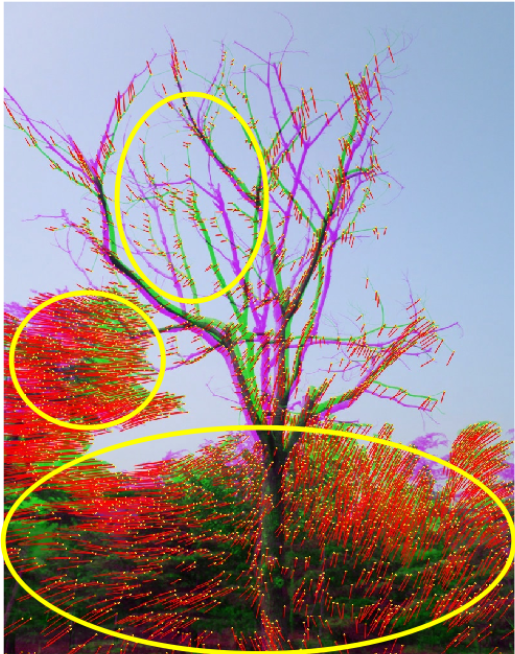
\includegraphics[height=10cm]{old.png}}\hspace{4em}
	\subfloat[改进的PyrLK光流法]{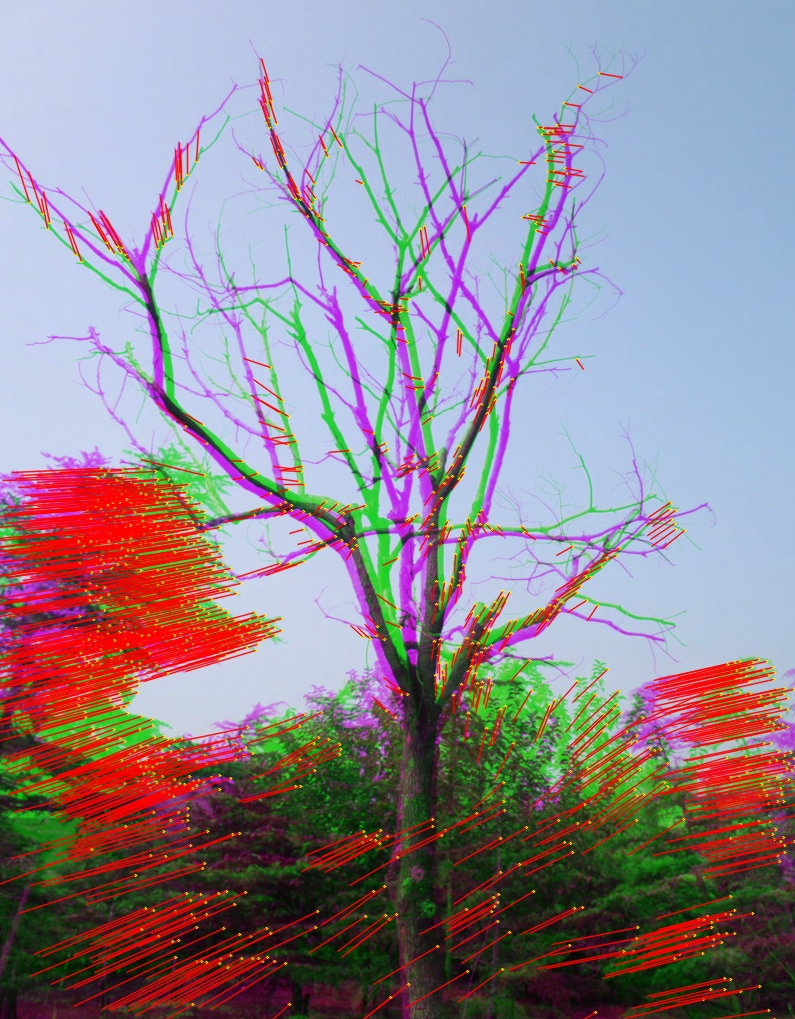
\includegraphics[height=10cm]{new.png}}
	\caption{支持仿射变换和提高鲁棒性的PyrLK光流法与传统光流法对比图}
	\label{fig:pyrlk}
\end{figure}


\clearpage
算法\ref{alg:pyrlk}给出了经过添加仿射变换支持和提高鲁棒性的PyrLK光流法算法的伪代码:\\
\begin{algorithm}[H]
	\caption{支持仿射变换和容错机制的PyrLK光流法}
	\label{alg:pyrlk}
	\begin{algorithmic}[1]
		\Require 图像$I$,$J$,图像$I$中的点$\mathbf{u}$
		\Ensure 图像$J$中对应点$\mathbf{v}$
		\State 构建图像$I$和$J$的金字塔表示: $\{I^L\}_{L=0,...,L_m}$和$\{J^L\}_{L=0,...,L_m}$
		\State 初始化金字塔估计值: $g^{L_{m}}=(g_x^{L_m}, g_y^{L_m})=(0,0)$
		\For{$L=L_m$to 0 with step of -1}
		\State 定位图像$I^L$上的点$\mathbf{u^L}$: $\mathbf{u}^L=(u_x,u_y)=\mathbf{u}/2^L$
		\State 设$\mathbf{a_1}=(a_{11},a_{12},a_{13})\quad \mathbf{a_2}=(a_{21},a_{22},a_{23})\quad 
				\mathbf{b}=(d_x^L, d_y^L, 1$
		\State 定义相似度:
				\[ \epsilon(\mathbf{d^L})=\epsilon(d_x,d_y)=\sum_{x=u_x-\omega_x}^{u_x+\omega_x}\sum_{y=u_y-\omega_y}
				^{u_y+\omega_y}(I(x,y) - J(x+\mathbf{a_1}\cdot \mathbf{b},y+\mathbf{a_2}\cdot \mathbf{b}))^2.\]
				\State 最小二乘法估计出$d^L$,使得$\epsilon $达到最小值
		\State L-1层金字塔估计值: $g^{L-1}=2(g^L+d^L)$
		\EndFor
		\State 最终光流向量: $\mathbf{d}=\mathbf{g^0}+\mathbf{d^0}$
		\State $\mathbf{v}=\mathbf{u+d}$
		\If{BackwardTrack$(\mathbf{v})$ = true}
			\If{MedianFilter$(\mathbf{v})$ = true}
				\State \Return $\mathbf{v}$
			\Else
				\State \Return NULL
			\EndIf
		\Else
			\State \Return NULL
		\EndIf
	\end{algorithmic}
\end{algorithm}

\section{本章小节}
\label{sec:conclusion}
本章首先介绍了光流法的由来,进而分析了LK光流法的思想和特点。然后对于基于图像金字塔的PyrLK光流法,它采用多分辨率图像层
来克服传统LK光流法无法捕捉图像中大块运动的缺陷。但是受缚于LK光流法的前提,该匹配算法只支持特征点的平移运动,由此带来很大
的束缚性。而且PyrLK光流法并没有对匹配的正确性进行验证,从而导致了很多错误的匹配对。基于这两方面的考虑,本章接着提出了支持
特征点旋转变换以及反向追踪的PyrLK光流法,这两个改进从根本上解决了PyrLK光流法的局限性,使PyrLK光流法的适用性和正确性都大大
的提升。本章的最后还给出了改进方法与传统方法的实验效果对比图。
